\documentclass[aspectratio=169]{beamer}

\usetheme{default}
\usepackage[utf8]{inputenc}
\usepackage[brazil]{babel}
\usepackage{tikz}
\usepackage{tabularx}
\usepackage{amsmath}
\usepackage{booktabs}
\usepackage{multirow}
\usepackage{graphicx}
\usepackage{hyperref}
\usepackage{amssymb}
\usepackage{colortbl}

% logos em presentation/imgs; figuras desta apresentação em ./figuras
\graphicspath{{../}{figuras/}}

\setbeamertemplate{footline}[frame number]
\setbeamertemplate{frametitle}[default][center]

\mode<presentation>{
\usetheme{Dresden}
\usecolortheme{seagull}
}

\setbeamertemplate{headline}{}

\definecolor{peeblue}{RGB}{1,123,165}
\definecolor{darkblue}{RGB}{0,65,115}

\setbeamercolor*{palette primary}{fg=black,bg=peeblue!80}
\setbeamercolor*{palette secondary}{fg=black,bg=peeblue!80!gray!80}
\setbeamercolor*{palette tertiary}{fg=black,bg=peeblue!100}
\setbeamercolor*{palette quaternary}{fg=black,bg=peeblue!110}

\usebackgroundtemplate
{%
    \begin{picture}(210,40)(-5,2)
    
\includegraphics[width=0.07\paperwidth,keepaspectratio]{imgs/pee-logo-short.png}
    \end{picture}%
}

\title{Reconhecimento Acústico de Alvos Submarinos no Dataset IARA}
\subtitle{Experimento mix\_small\_medium: Uma Classe para os Navios Abaixo de 100 m}
\author{Evandro Rocha}
\date{Novembro de 2026}

\institute
{
  Universidade Federal do Rio de Janeiro\\
  UFRJ / COPPE / PEE
}

\newcommand{\cahi}[1]{\cellcolor{green!30}\textbf{#1}}
\newcommand{\calo}[1]{\cellcolor{red!20}#1}
\newcommand{\camd}[1]{\cellcolor{yellow!35}#1}
\newcommand{\mix}{\texttt{MIX\_SMALL\_MEDIUM}}

\begin{document}

{
\usebackgroundtemplate{
    \begin{picture}(210,55)(-5,0)
    
\includegraphics[height=0.14\paperwidth,keepaspectratio]{imgs/pee-logo.png}
    \end{picture}%
    \begin{picture}(210,55)(-28,2)
    
\includegraphics[height=0.14\paperwidth,keepaspectratio]{imgs/coppe-logo.pdf}
    \end{picture}
}
\begin{frame}
  \bigskip\bigskip\bigskip\bigskip
  \titlepage
\end{frame}
}

\begin{frame}{Agenda da Apresentação}
  \footnotesize
  \setbeamercolor{block title}{bg=darkblue,fg=white}
  \setbeamercolor{block body}{bg=peeblue!8,fg=black}
  \setbeamertemplate{section in toc}{%
    \vspace{0.14cm}%
    \leavevmode%
    \tikz[baseline=-0.65ex]\node[circle,fill=peeblue,text=white,inner sep=0pt,font=\tiny\bfseries,minimum size=1.35em]{\inserttocsectionnumber};%
    \hspace{0.35em}%
    \inserttocsection\par%
  }
  \begin{columns}[t]
      \begin{column}{0.6\textwidth}
          \begin{block}{\small\textbf{Experimento mix\_small\_medium}}
              \tableofcontents
          \end{block}
      \end{column}
  \end{columns}
\end{frame}

\begin{frame}{Resumo}
    \footnotesize
    \begin{block}{\small Pergunta: se SMALL e MEDIUM forem uma só classe, o modelo a reconhece em navios novos?}
        \scriptsize
        \begin{enumerate}
            \setlength{\itemsep}{3pt}
            \item \textbf{Sim.} Em navios nunca vistos, o recall de \mix{} é \textbf{76\%} (82\% no split por gravação). Perda de só 6 pontos; com as classes do IARA, MEDIUM perdia $\sim$31.
            \item \textbf{Split por navio: SP 74,5, ACC 74,6} (acaso 33\%).
            \item \textbf{Treinar com os rótulos novos dá o mesmo que juntar as previsões} do modelo de 4 classes (p = 0,50). O modelo já sabia ``navio $<$ 100 m''; não sabia separar SMALL de MEDIUM.
            \item \textbf{Os erros agora estão na fronteira de 100 m:} LARGE de 100--150 m vira \mix{} em 52\% das gravações; acima de 250 m, em 22\%. Aqui há gradiente de tamanho.
            \item \textbf{A razão está no som:} navios $<$ 100 m têm o pico entre 90 e 221 Hz; LARGE, abaixo de 90 Hz, e esse grave cresce no CPA. Entre SMALL e MEDIUM, nenhuma faixa difere (0 de 140 testes).
        \end{enumerate}
    \end{block}
    \begin{alertblock}{\small Atenção}
        \scriptsize
        Com 3 classes o acaso é 33\% (com as classes do IARA, 25\%). \textbf{O SP deste experimento não é comparável ao SP do artigo}: é um diagnóstico de até onde o IARA permite generalizar hoje.
    \end{alertblock}
\end{frame}

%===========================================
\section{O Experimento}

\begin{frame}
    \centering
    \huge O Experimento
\end{frame}

\begin{frame}{Motivação: SMALL e MEDIUM se Confundem em Navios Novos}
    \footnotesize
    \begin{block}{\small MLP LOFAR do NB29, classes do IARA, split por navio (\% da classe verdadeira)}
        \scriptsize
        \centering
        \setlength{\tabcolsep}{6pt}
        \begin{tabular}{lcccc}
        \toprule
        Verdadeira $\backslash$ Prevista & SMALL & MEDIUM & LARGE & BACKGROUND \\
        \midrule
        SMALL & \camd{49,0} & 22,9 & 23,9 & 4,2 \\
        MEDIUM & \calo{51,0} & 32,3 & 15,3 & 1,4 \\
        LARGE & 20,3 & 10,5 & 67,7 & 1,6 \\
        BACKGROUND & 11,3 & 4,3 & 3,3 & 81,1 \\
        \bottomrule
        \end{tabular}
    \end{block}
    \vspace{0.1cm}
    \begin{alertblock}{Leitura}
        \scriptsize
        Uma MEDIUM de navio novo é prevista SMALL em \textbf{51\%} dos casos, tanto quanto uma SMALL (49\%). Mas SMALL e MEDIUM quase nunca viram BACKGROUND (4\% e 1\%). O modelo parece ter aprendido ``navio menor'' sem saber dizer se é SMALL ou MEDIUM.
    \end{alertblock}
\end{frame}

\begin{frame}{Classes e Modelo do Experimento mix\_small\_medium}
    \footnotesize
    \begin{columns}[t]
        \column{0.62\textwidth}
        \begin{block}{\small Classes}
            \tiny
            \centering
            \setlength{\tabcolsep}{3pt}
            \begin{tabular}{lccc}
            \toprule
             & \mix & LARGE & BACKGROUND \\
            \midrule
            Inclui & SMALL + MEDIUM & LARGE & BACKGROUND \\
            Comprimento & 8--98 m & 100--349 m & -- \\
            Gravações & 873 & 572 & 261 \\
            Horas & 66,8 & 44,2 & 10,9 \\
            Navios distintos & 169 & 417 & -- \\
            Nº efetivo de navios & \camd{24,3} & 213,6 & -- \\
            \bottomrule
            \end{tabular}
        \end{block}
        \column{0.36\textwidth}
        \begin{block}{\small Modelo}
            \scriptsize
            \begin{itemize}
                \setlength{\itemsep}{1pt}
                \item MLP h32-16 \textbf{treinada do zero} com os 3 rótulos acima.
                \item Mesma arquitetura, hiperparâmetros, folds e sementes da MLP LOFAR do NB29: \textbf{só as classes mudam}.
                \item Dois splits: por gravação (artigo) e por navio.
            \end{itemize}
        \end{block}
    \end{columns}
    \vspace{0.1cm}
    \begin{alertblock}{Leitura}
        \scriptsize
        Juntar as classes dobra a diversidade de navios (de $\sim$12 para 24 navios efetivos), mas \mix{} continua bem abaixo de LARGE: lanchas de prático e dragas HANG BO ainda dominam.
    \end{alertblock}
\end{frame}

%===========================================
\section{Resultados}

\begin{frame}
    \centering
    \huge Resultados
\end{frame}

\begin{frame}{\mix{} Generaliza para Navios Novos}
    \begin{columns}[c]
        \column{0.56\textwidth}
        \centering
        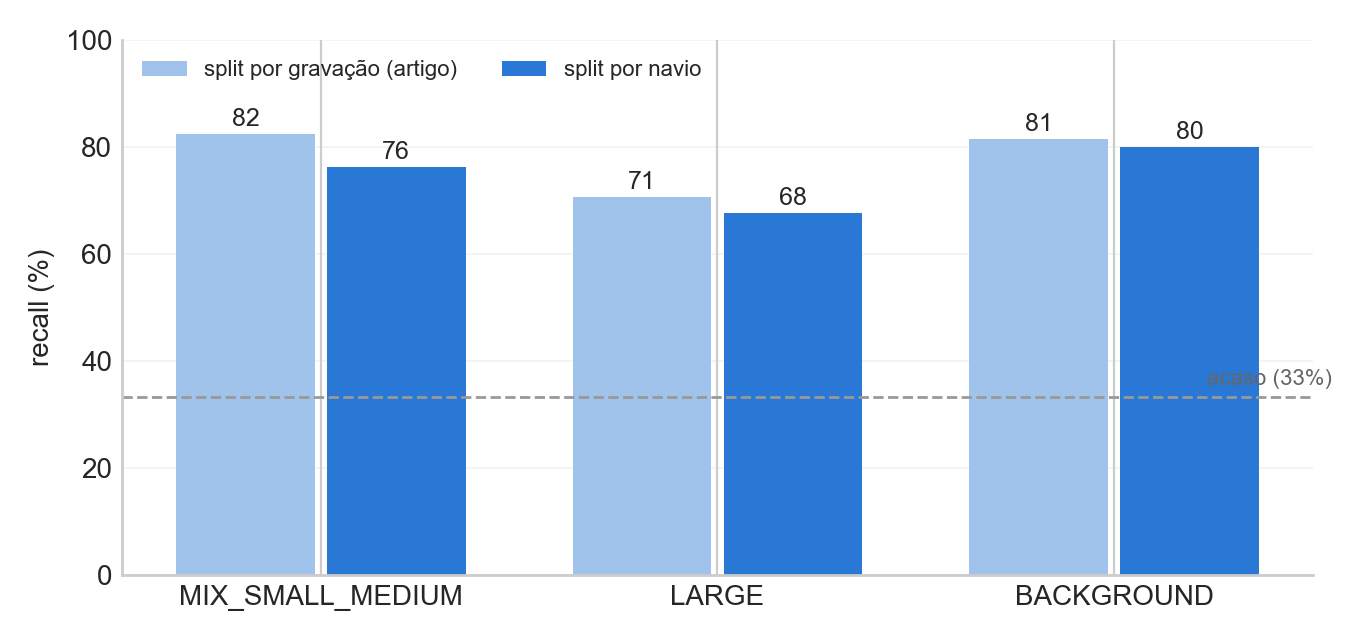
\includegraphics[width=\textwidth]{recall_splits.png}
        \column{0.42\textwidth}
        \begin{block}{\small MLP mix\_small\_medium}
            \tiny
            \centering
            \setlength{\tabcolsep}{3pt}
            \begin{tabular}{lccc}
            \toprule
             & gravação & navio & queda \\
            \midrule
            SP & 78,0 & \cahi{74,5} & 3,6 \\
            ACC & 78,2 & \cahi{74,6} & 3,5 \\
            \mix & 82,4 & 76,2 & 6,1 \\
            LARGE & 70,6 & 67,7 & 2,9 \\
            BACKGROUND & 81,5 & 79,9 & 1,5 \\
            \bottomrule
            \end{tabular}

            \vspace{0.05cm}
            {\tiny Média de 10 folds; desvio de SP e ACC $\leq$ 1,0.\par}
        \end{block}
    \end{columns}
    \vspace{0.05cm}
    \begin{alertblock}{Leitura}
        \scriptsize
        Em navios nunca vistos, \mix{} acerta \textbf{76\%}, perdendo só 6 pontos em relação ao split por gravação. Com as classes do IARA, o recall de MEDIUM caía de $\sim$66\% para $\sim$35\%. \textbf{O modelo reconhece ``navio $<$ 100 m'' em navios novos.}
    \end{alertblock}
\end{frame}

\begin{frame}{Treinar com os Rótulos Novos Ensina Algo a Mais?}
    \footnotesize
    \begin{table}
    \centering
    \scriptsize
    \setlength{\tabcolsep}{4pt}
    \begin{tabular}{llccccc}
    \toprule
    Split & Modelo & SP & ACC & \mix & LARGE & BACKGROUND \\
    \midrule
    \multirow{2}{*}{por navio} & MLP mix\_small\_medium & 74,5 & 74,6 & 76,2 & 67,7 & 79,9 \\
     & MLP do NB29, juntada depois & 75,0 & 75,1 & 76,6 & 67,7 & 81,1 \\
    \midrule
    \multirow{2}{*}{por gravação} & MLP mix\_small\_medium & 78,0 & 78,1 & 82,4 & 70,6 & 81,5 \\
     & MLP do NB29, juntada depois & 77,7 & 77,8 & 82,3 & 71,2 & 80,0 \\
    \bottomrule
    \end{tabular}
    \end{table}
    {\tiny ``Juntada depois'' = MLP treinada com as classes do IARA; as previsões SMALL e MEDIUM viram \mix{} depois do treino.\par}
    \vspace{0.1cm}
    \begin{block}{\small Diferença (mix\_small\_medium $-$ juntada), teste F 5x2cv}
        \scriptsize
        Split por navio: $\Delta$ ACC $-$0,52 (p = 0,50, melhor em 3 de 10 folds). \quad Split por gravação: $\Delta$ ACC +0,31 (p = 0,72).
    \end{block}
    \begin{alertblock}{Leitura}
        \scriptsize
        \textbf{Não.} Os dois dão o mesmo resultado. O modelo das 4 classes do IARA já separava ``navio $<$ 100 m'' de LARGE e de BACKGROUND; o que ele não conseguia era a divisão interna entre SMALL e MEDIUM.
    \end{alertblock}
\end{frame}

\begin{frame}{Matrizes de Confusão}
    \footnotesize
    \begin{columns}[t]
        \column{0.49\textwidth}
        \begin{block}{\small Split por navio (\% da verdadeira)}
            \tiny
            \centering
            \setlength{\tabcolsep}{3pt}
            \begin{tabular}{lccc}
            \toprule
            Verd. $\backslash$ Prev. & \mix & LARGE & BG \\
            \midrule
            \mix & \cahi{76,2} & 21,3 & 2,5 \\
            LARGE & \calo{30,9} & 67,6 & 1,6 \\
            BACKGROUND & 15,9 & 4,1 & 79,9 \\
            \bottomrule
            \end{tabular}
        \end{block}
        \column{0.49\textwidth}
        \begin{block}{\small Split por gravação (\% da verdadeira)}
            \tiny
            \centering
            \setlength{\tabcolsep}{3pt}
            \begin{tabular}{lccc}
            \toprule
            Verd. $\backslash$ Prev. & \mix & LARGE & BG \\
            \midrule
            \mix & 82,4 & 15,6 & 2,0 \\
            LARGE & 27,8 & 70,6 & 1,6 \\
            BACKGROUND & 15,0 & 3,5 & 81,5 \\
            \bottomrule
            \end{tabular}
        \end{block}
    \end{columns}
    \vspace{0.15cm}
    \begin{alertblock}{Leitura}
        \scriptsize
        O erro principal é a troca entre \mix{} e LARGE: em navios novos, 21\% das \mix{} vão para LARGE e 31\% das LARGE vão para \mix. BACKGROUND quase não vira LARGE, mas 16\% dele é previsto \mix.
    \end{alertblock}
\end{frame}

%===========================================
\section{Onde o Modelo Erra}

\begin{frame}
    \centering
    \huge Onde o Modelo Erra
\end{frame}

\begin{frame}{Recall de \mix{} por Tipo de Navio}
    \footnotesize
    \begin{columns}[t]
        \column{0.55\textwidth}
        \begin{block}{\small Por tipo}
            \scriptsize
            \centering
            \setlength{\tabcolsep}{3pt}
            \begin{tabular}{llcc}
            \toprule
            Classe IARA & Tipo (navios) & Acerto & Prev. LARGE \\
            \midrule
            \multirow{4}{*}{SMALL} & Prático (15) & 71 & 25 \\
             & Rebocador (34) & 71 & 26 \\
             & Pesca (22) & \camd{68} & 29 \\
             & Outros (16) & 86 & 14 \\
            \midrule
            \multirow{3}{*}{MEDIUM} & Draga HANG BO (3) & 82 & 17 \\
             & OSS (46) & 84 & 15 \\
             & Outros supply/AHTS (33) & 77 & 21 \\
            \bottomrule
            \end{tabular}
        \end{block}
        \column{0.43\textwidth}
        \begin{block}{\small Pela classe original}
            \scriptsize
            \centering
            \begin{tabular}{lcc}
            \toprule
             & Acerto & Prev. LARGE \\
            \midrule
            SMALL & 72 & 24 \\
            MEDIUM & 81 & 18 \\
            \bottomrule
            \end{tabular}
        \end{block}
    \end{columns}
    \vspace{0.1cm}
    \begin{alertblock}{Leitura}
        \scriptsize
        Todos os tipos ficam acima de 65\%, inclusive os com poucos navios. A parte SMALL erra mais, e quase sempre para LARGE: é o mesmo padrão das lanchas de prático com graves fortes (NB39). O erro é LARGE, não BACKGROUND.
    \end{alertblock}
\end{frame}

\begin{frame}{A Nova Fronteira: 100 m}
    \begin{columns}[c]
        \column{0.6\textwidth}
        \centering
        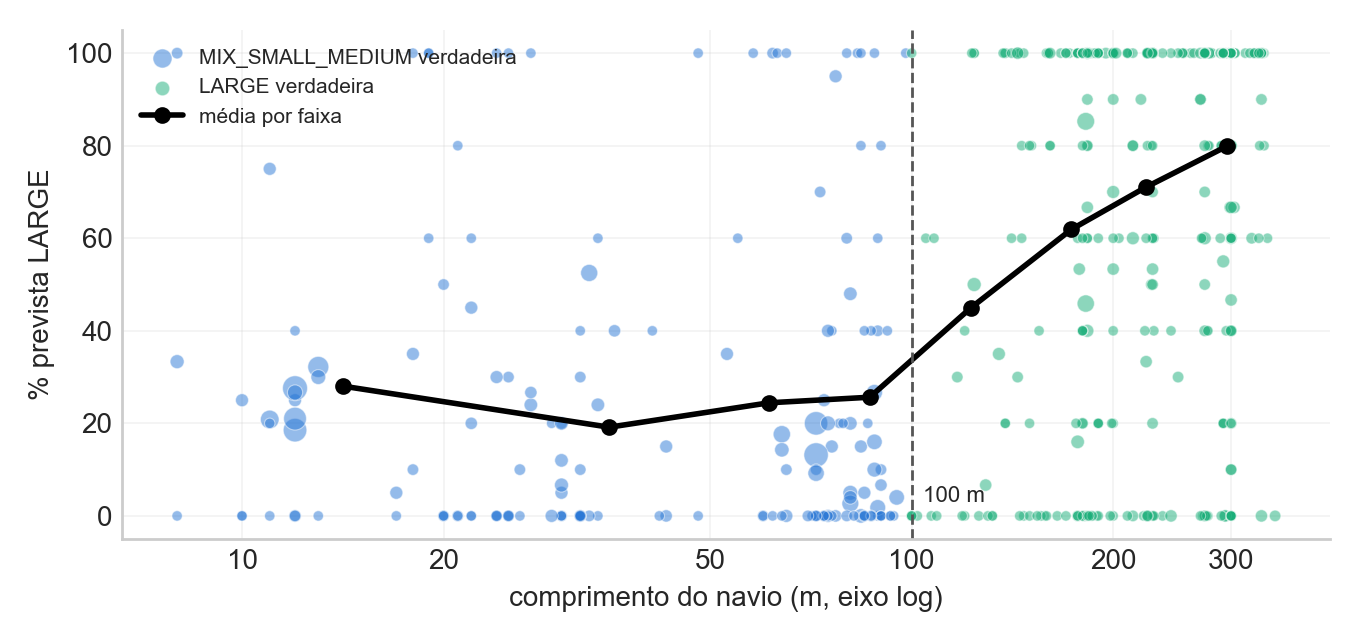
\includegraphics[width=\textwidth]{fronteira_100m.png}

        {\tiny Um ponto por navio (tamanho = nº de gravações); split por navio.\par}
        \column{0.38\textwidth}
        \begin{block}{\small LARGE prevista \mix}
            \scriptsize
            \centering
            \begin{tabular}{lcc}
            \toprule
            Comprimento & Navios & \% \\
            \midrule
            100--150 m & 39 & \calo{52} \\
            150--200 m & 103 & 36 \\
            200--250 m & 80 & 33 \\
            250--400 m & 195 & 22 \\
            \bottomrule
            \end{tabular}
        \end{block}
    \end{columns}
    \vspace{0.05cm}
    \begin{alertblock}{Leitura}
        \scriptsize
        \textbf{Acima de 100 m há um gradiente de tamanho:} quanto maior o navio, mais ele é previsto LARGE. Na fronteira de 50 m (SMALL $\times$ MEDIUM) não havia gradiente nenhum. Abaixo de 100 m, a \% prevista LARGE fica em 20--28\% em todos os comprimentos.
    \end{alertblock}
\end{frame}

%===========================================
\section{\texorpdfstring{Por que \texttt{MIX\_SMALL\_MEDIUM} e LARGE se Separam}{Por que MIX e LARGE se Separam}}

\begin{frame}
    \centering
    \huge Por que \texttt{MIX\_SMALL\_MEDIUM}\\[0.2cm] e LARGE se Separam
\end{frame}

\begin{frame}{Como Medimos: Fatias Alinhadas pelo CPA}
    \footnotesize
    \begin{columns}[t]
        \column{0.52\textwidth}
        \begin{block}{\small Procedimento}
            \scriptsize
            \begin{itemize}
                \setlength{\itemsep}{2pt}
                \item Só gravações \textbf{com CPA} (A e C): 797 gravações.
                \item LOFAR (dB acima do fundo TPSW) cortado em \textbf{10 fatias de 30 s}, de $-$150 s a +150 s do CPA.
                \item Cada fatia resumida em \textbf{14 faixas} de 15 Hz a 8 kHz.
                \item \textbf{Um ponto por navio} (média das suas gravações).
                \item 140 testes por par de classes (fatia $\times$ faixa), com correção para testes múltiplos (FDR).
            \end{itemize}
        \end{block}
        \column{0.46\textwidth}
        \begin{block}{\small Como ler a AUC}
            \scriptsize
            Sorteio um navio de cada classe e vejo qual tem mais energia na faixa. A AUC é a \% das comparações que a 2ª classe ganha.
            \begin{itemize}
                \setlength{\itemsep}{1pt}
                \item \textbf{50\%:} empate (cara ou coroa); a faixa não separa as classes.
                \item \textbf{Perto de 100\%:} a 2ª classe quase sempre tem mais.
                \item \textbf{Perto de 0\%:} a 1ª classe quase sempre tem mais.
            \end{itemize}
            ``Empate'' não é energia igual: os dois grupos têm a mesma variedade de valores.
        \end{block}
    \end{columns}
\end{frame}

\begin{frame}{SMALL e MEDIUM Empatam; LARGE se Separa dos Dois}
    \footnotesize
    \begin{columns}[t]
        \column{0.34\textwidth}
        \begin{block}{\small Diferenças confiáveis (de 140)}
            \scriptsize
            \centering
            \begin{tabular}{lc}
            \toprule
            SMALL $\times$ MEDIUM & \calo{0} \\
            MEDIUM $\times$ LARGE & \cahi{91} \\
            SMALL $\times$ LARGE & \cahi{100} \\
            \bottomrule
            \end{tabular}

            \vspace{0.05cm}
            {\tiny Só por acaso, $\sim$7 teriam p $<$ 0,05.\par}
        \end{block}
        \column{0.64\textwidth}
        \begin{block}{\small Quem tem mais energia (\% das comparações que ganha)}
            \tiny
            \centering
            \setlength{\tabcolsep}{3pt}
            \begin{tabular}{lccc}
            \toprule
            Faixa & SMALL $\times$ MEDIUM & MEDIUM $\times$ LARGE & SMALL $\times$ LARGE \\
            \midrule
            23--37 Hz & empate & LARGE 54--66 & LARGE 70--76 \\
            \textbf{37--58 Hz} & empate & \textbf{LARGE 75--82} & \textbf{LARGE 75--85} \\
            58--90 Hz & empate & LARGE 64--79 & LARGE 57--74 \\
            90--141 Hz & empate & MEDIUM 61--69 & SMALL 62--71 \\
            \textbf{141--221 Hz} & empate & \textbf{MEDIUM 70--79} & \textbf{SMALL 70--76} \\
            5--8 kHz & empate & LARGE 72--77 & LARGE 60--67 \\
            \bottomrule
            \end{tabular}

            \vspace{0.05cm}
            {\tiny Intervalo = variação ao longo das 10 fatias da passagem.\par}
        \end{block}
    \end{columns}
    \vspace{0.05cm}
    \begin{alertblock}{Leitura}
        \scriptsize
        \textbf{SMALL e MEDIUM diferem de LARGE do mesmo jeito:} LARGE tem mais energia abaixo de $\sim$90 Hz; os navios $<$ 100 m, entre 90 e 221 Hz. Por isso juntar SMALL e MEDIUM funciona. Entre SMALL e MEDIUM, nenhuma faixa difere. Nos agudos as diferenças em dB são minúsculas: quem separa são os graves.
    \end{alertblock}
\end{frame}

\begin{frame}{Ao Longo da Passagem}
    \centering
    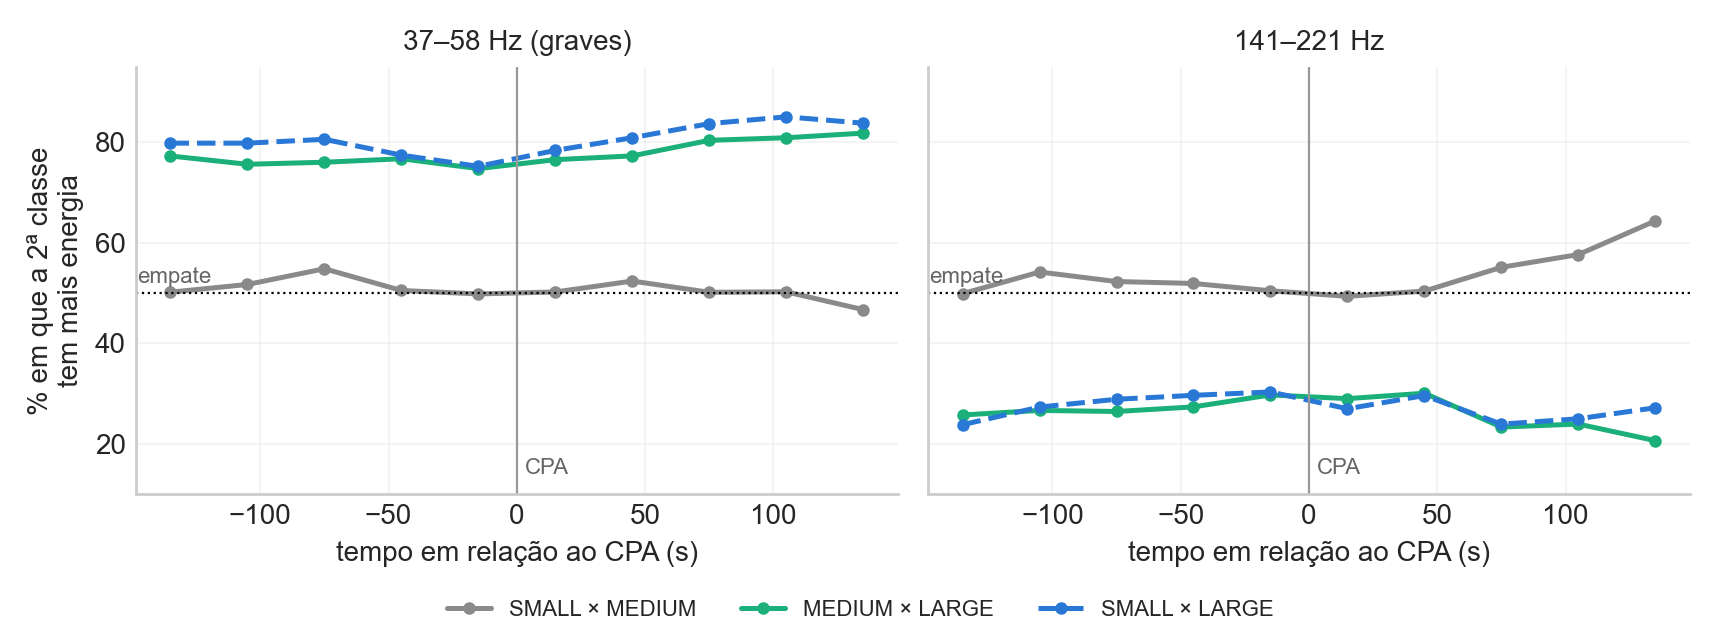
\includegraphics[width=0.86\textwidth]{auc_passagem.png}
    \vspace{-0.05cm}
    \begin{alertblock}{Leitura}
        \scriptsize
        Nos graves, os LARGE ganham em 75--85\% das comparações \textbf{em toda a passagem}, e a vantagem \textbf{cresce depois do CPA}, como se espera do som do próprio navio. SMALL $\times$ MEDIUM fica em torno do empate o tempo todo.
    \end{alertblock}
\end{frame}

\begin{frame}{A Diferença MEDIUM $\times$ LARGE Não é Acaso}
    \footnotesize
    \begin{table}
    \centering
    \tiny
    \setlength{\tabcolsep}{3pt}
    \begin{tabular}{llcccccc}
    \toprule
    Faixa & Momento & AUC real & Rótulos embaralhados & Mesmo sentido nas metades & p$<$0,05 na outra metade & Só A & Só C \\
    \midrule
    37--58 Hz & perto do CPA & 75 & 42--58 & 100\% & 100\% & 80 & 71 \\
    37--58 Hz & depois do CPA & 81 & 41--58 & 100\% & 100\% & 86 & 76 \\
    141--221 Hz & perto do CPA & 30 & 42--58 & 100\% & 100\% & 27 & 34 \\
    5--8 kHz & perto do CPA & 77 & 42--58 & 100\% & 100\% & 78 & 78 \\
    \bottomrule
    \end{tabular}
    \end{table}
    {\tiny AUC = \% em que LARGE tem mais energia. Embaralhado: 95\% central de 1000 sorteios. Metades: 100 divisões dos navios em duas metades sem navio em comum.\par}
    \vspace{0.1cm}
    \begin{columns}[t]
        \column{0.49\textwidth}
        \begin{block}{\small Descartado}
            \scriptsize
            \begin{itemize}
                \setlength{\itemsep}{1pt}
                \item \textbf{Acaso:} o embaralhado nunca chegou ao real.
                \item \textbf{Poucos navios:} se repete em metades independentes.
                \item \textbf{Distância:} aparece em A (85/140) e em C (59/140).
            \end{itemize}
        \end{block}
        \column{0.49\textwidth}
        \begin{alertblock}{\small Não descartado}
            \scriptsize
            Parte da diferença pode vir de algo que anda junto com o tamanho: \textbf{tipo de navio} (LARGE é quase todo carga e petroleiro; MEDIUM, apoio offshore), velocidade ou condições de gravação.
        \end{alertblock}
    \end{columns}
\end{frame}

\begin{frame}{Faixa de Pico de Cada Classe}
    \centering
    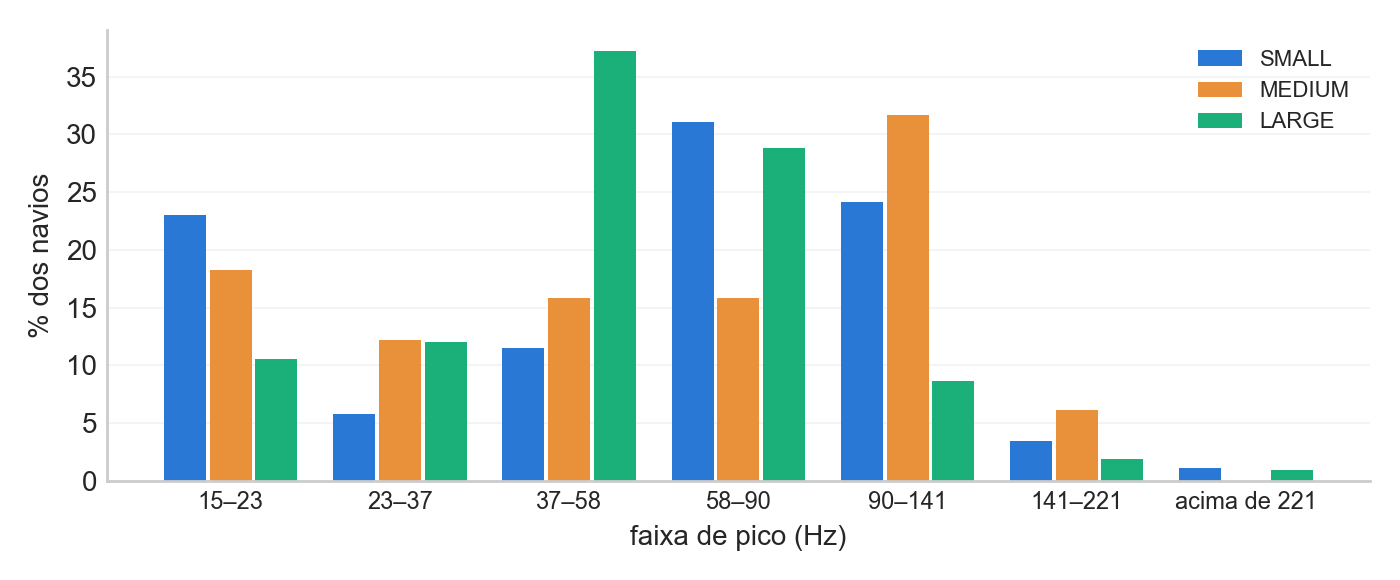
\includegraphics[width=0.78\textwidth]{pico_classes.png}

    {\tiny Faixa de pico = das 14 faixas, a de maior energia média (LOFAR médio da gravação inteira, A--D). 15--23 Hz é uma única linha do LOFAR e sofre com ruído de fundo.\par}
    \vspace{0.05cm}
    \begin{alertblock}{Leitura}
        \scriptsize
        \textbf{LARGE concentra o pico em 37--90 Hz} (66\% dos navios; só 9\% em 90--141 Hz). Entre os MEDIUM, a faixa mais comum é \textbf{90--141 Hz} (32\%). Os SMALL se espalham, e o pico mais comum (58--90 Hz) é \emph{mais grave} que o do MEDIUM: entre SMALL e MEDIUM, o tamanho não acompanha a frequência.
    \end{alertblock}
\end{frame}

\begin{frame}{O Grave dos LARGE Depende do CPA; o dos Menores, Não}
    \footnotesize
    \begin{columns}[c]
        \column{0.5\textwidth}
        \centering
        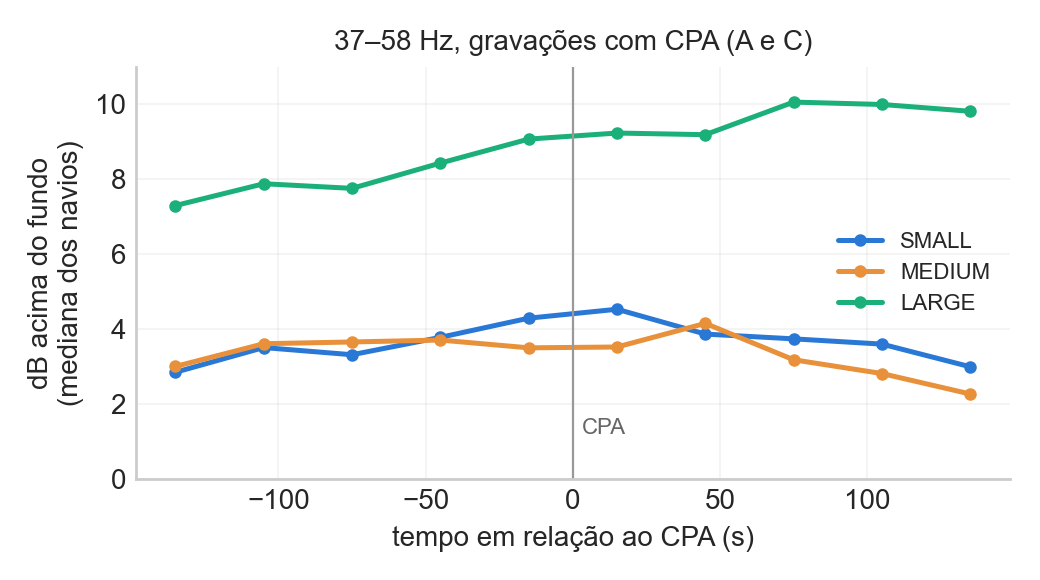
\includegraphics[width=\textwidth]{energia_passagem.png}
        \column{0.48\textwidth}
        \begin{block}{\small \% das gravações com pico em 37--90 Hz}
            \tiny
            \centering
            \setlength{\tabcolsep}{4pt}
            \begin{tabular}{lcccc}
            \toprule
             & A & B & C & D \\
             & CPA & sem & CPA & sem \\
            \midrule
            SMALL & 44 & 33 & 54 & 41 \\
            MEDIUM & 29 & 38 & 47 & 26 \\
            LARGE & \cahi{69} & \calo{33} & \cahi{76} & 55 \\
            \bottomrule
            \end{tabular}
        \end{block}
        \begin{block}{\small Mesmo navio, com e sem CPA}
            \tiny
            \centering
            \begin{tabular}{lccc}
            \toprule
             & Navios & Sobe & Cai \\
            \midrule
            SMALL & 32 & 13 & 10 \\
            MEDIUM & 28 & 8 & 11 \\
            LARGE & 27 & \cahi{12} & 3 \\
            \bottomrule
            \end{tabular}
        \end{block}
    \end{columns}
    \begin{alertblock}{Leitura}
        \scriptsize
        Nos LARGE, o grave sobe $\sim$3 dB na passagem e \textbf{continua alto depois do CPA}. Em SMALL e MEDIUM há só um ``morrinho'' de 1--1,5 dB que volta logo. \textbf{Sem CPA, os LARGE perdem o pico grave e ficam parecidos com os navios $<$ 100 m}: é onde a MLP mais erra LARGE.
    \end{alertblock}
\end{frame}

\begin{frame}{Cada Navio MEDIUM contra Todas as Gravações LARGE (37--58 Hz)}
    \footnotesize
    \begin{columns}[t]
        \column{0.55\textwidth}
        \begin{block}{\small Faixa de pico do navio MEDIUM $\times$ quanto ele se parece com LARGE}
            \tiny
            \centering
            \setlength{\tabcolsep}{3pt}
            \begin{tabular}{lccc}
            \toprule
            Faixa de pico & Mais grave que & Intermediário & Bem abaixo \\
             & a maioria dos LARGE & (50--80\% acima) & ($>$80\% acima) \\
            \midrule
            15--23 Hz & 1 & 3 & 11 \\
            23--37 Hz & \camd{4} & \camd{5} & 1 \\
            37--58 Hz & \camd{5} & \camd{8} & 0 \\
            58--90 Hz & 3 & 1 & 9 \\
            90--141 Hz & 0 & 0 & \cahi{26} \\
            141--221 Hz & 0 & 0 & \cahi{5} \\
            \bottomrule
            \end{tabular}
        \end{block}
        \column{0.43\textwidth}
        \begin{block}{\small Números}
            \scriptsize
            \begin{itemize}
                \setlength{\itemsep}{1pt}
                \item 82 navios MEDIUM $\times$ 572 gravações LARGE.
                \item Mediana: LARGE 7,7 dB; MEDIUM 3,8 dB.
                \item \textbf{69 de 82} navios MEDIUM ficam abaixo da maioria dos LARGE.
                \item HELEN (transporte de gado, 80 m) tem mais grave que \textbf{todas} as 572 gravações LARGE.
            \end{itemize}
        \end{block}
    \end{columns}
    \vspace{0.05cm}
    \begin{alertblock}{Leitura}
        \scriptsize
        \textbf{Onde fica o pico importa:} os 31 navios MEDIUM com pico entre 90 e 221 Hz ficam todos bem abaixo dos LARGE. Os que têm pico entre 23 e 58 Hz soam ``como LARGE'' (HELEN, o pesqueiro HELLAS TUNA, as dragas HANG BO): são os candidatos a erro \mix{} $\rightarrow$ LARGE.
    \end{alertblock}
\end{frame}

\begin{frame}{Dragas HANG BO: Provavelmente Navios Gêmeos}
    \footnotesize
    \begin{columns}[t]
        \column{0.52\textwidth}
        \begin{block}{\small Os dois navios}
            \tiny
            \centering
            \setlength{\tabcolsep}{3pt}
            \begin{tabular}{lcc}
            \toprule
             & HANG BO 2002 & HANG BO 2003 \\
            \midrule
            ID & 237 & 238 \\
            Tipo & Motor Hopper & Motor Hopper \\
            Comprimento & 72 m & 72 m \\
            Gravações & 67 & 79 \\
            Energia 37--58 Hz & 6,6 dB & 6,5 dB \\
            Faixa de pico & 23--37 Hz & 23--37 Hz \\
            \bottomrule
            \end{tabular}
        \end{block}
        \begin{block}{\small Peso na classe}
            \scriptsize
            146 das 397 gravações MEDIUM (\textbf{37\%}); o 3º navio MEDIUM com mais gravações tem só 17.
        \end{block}
        \column{0.46\textwidth}
        \begin{block}{\small Folds do split por navio}
            \tiny
            \centering
            \begin{tabular}{lc}
            \toprule
            Situação & Folds \\
            \midrule
            Os dois no treino & 0, 5, 8 \\
            Os dois no teste & 1, 4, 9 \\
            \calo{Um no treino, o outro no teste} & \calo{2, 3, 6, 7} \\
            \bottomrule
            \end{tabular}
        \end{block}
    \end{columns}
    \vspace{0.05cm}
    \begin{alertblock}{Leitura}
        \scriptsize
        Mesmo tipo, comprimento, nomes em sequência e quase a mesma assinatura: provavelmente construídos em série (inferência pelos dados, não confirmada em registro). Em \textbf{4 dos 10 folds}, o modelo treina com um e é testado no outro: parte do acerto em MEDIUM no split por navio pode estar inflada.
    \end{alertblock}
\end{frame}

%===========================================
\section{Conclusões}

\begin{frame}
    \centering
    \huge Conclusões
\end{frame}

\begin{frame}{Conclusões}
    \footnotesize
    \begin{block}{\small O que o experimento mix\_small\_medium mostra}
        \scriptsize
        \begin{enumerate}
            \setlength{\itemsep}{0.5pt}
            \item \textbf{O IARA sustenta ``navio $<$ 100 m $\times$ navio $\geq$ 100 m $\times$ mar'' em navios novos}: SP 74,5 e ACC 74,6 com split por navio, perdendo só 3,5 pontos de ACC em relação ao split por gravação.
            \item \textbf{A dificuldade está em separar SMALL de MEDIUM}, não em reconhecer navios menores: treinar com \mix{} não ensina nada que o modelo das 4 classes já não soubesse. Com os navios que existem, o IARA separa porte grosso.
            \item \textbf{Os erros que restam} estão nos LARGE de 100--150 m e nas SMALL com graves fortes.
            \item \textbf{Há base acústica para a fronteira de 100 m, não para a de 50 m:} navios $<$ 100 m têm o pico entre 90 e 221 Hz; LARGE, abaixo de 90 Hz, e esse grave cresce no CPA. SMALL $\times$ MEDIUM: 0 diferenças em 140 testes.
            \item \textbf{Erros de LARGE vêm das gravações sem CPA} (o pico grave some); \textbf{erros de \mix{} vêm de navios com pico abaixo de 58 Hz}.
            \item \textbf{Dragas HANG BO}, provavelmente gêmeas, separadas entre treino e teste em 4 dos 10 folds.
        \end{enumerate}
    \end{block}
    \begin{alertblock}{\small Cuidados}
        \scriptsize
        A tarefa é mais fácil (3 classes, acaso 33\%): o SP não substitui o do artigo. A classe se chama \mix{} para não ser confundida com SMALL. Resultado só com a MLP; falta repetir em outros modelos.
    \end{alertblock}
\end{frame}

\end{document}
